\section{Results}\label{sec:results}

\subsection{Participants}

We recruited a total of 18 participants for our study using posters we placed on the university campus in combination with snowball sampling.
Participants age ranged from 18 to 59 years and only 3 of the 18 participants identified as female, all others identified as male.
Each participant received a compensation of \euro10.00 for their efforts.
The study was conducted from November to December, but except for temperature differences and some light raining, general weather conditions were consistent between study sessions.
Each session to about 90 minutes in total.
We experienced no study cancellations and all recorded data was useable.

\subsection{Route Data}

In this section we describe the evaluation of the quantitative ratings performed by participants on the measure of “Travel satisfaction, based on the road” using the \likertshift, \audiorecording, and \mapping methods respectively, as described in \autoref{subsec:recording_methods} and \autoref{subsec:data_collection}. \autoref{fig:route_ratings} shows a visually appealing overview of all data collected using all three methods.

\begin{figure}[!htb]
    \centering
    \begin{subfigure}{.3333\textwidth}
        \centering
        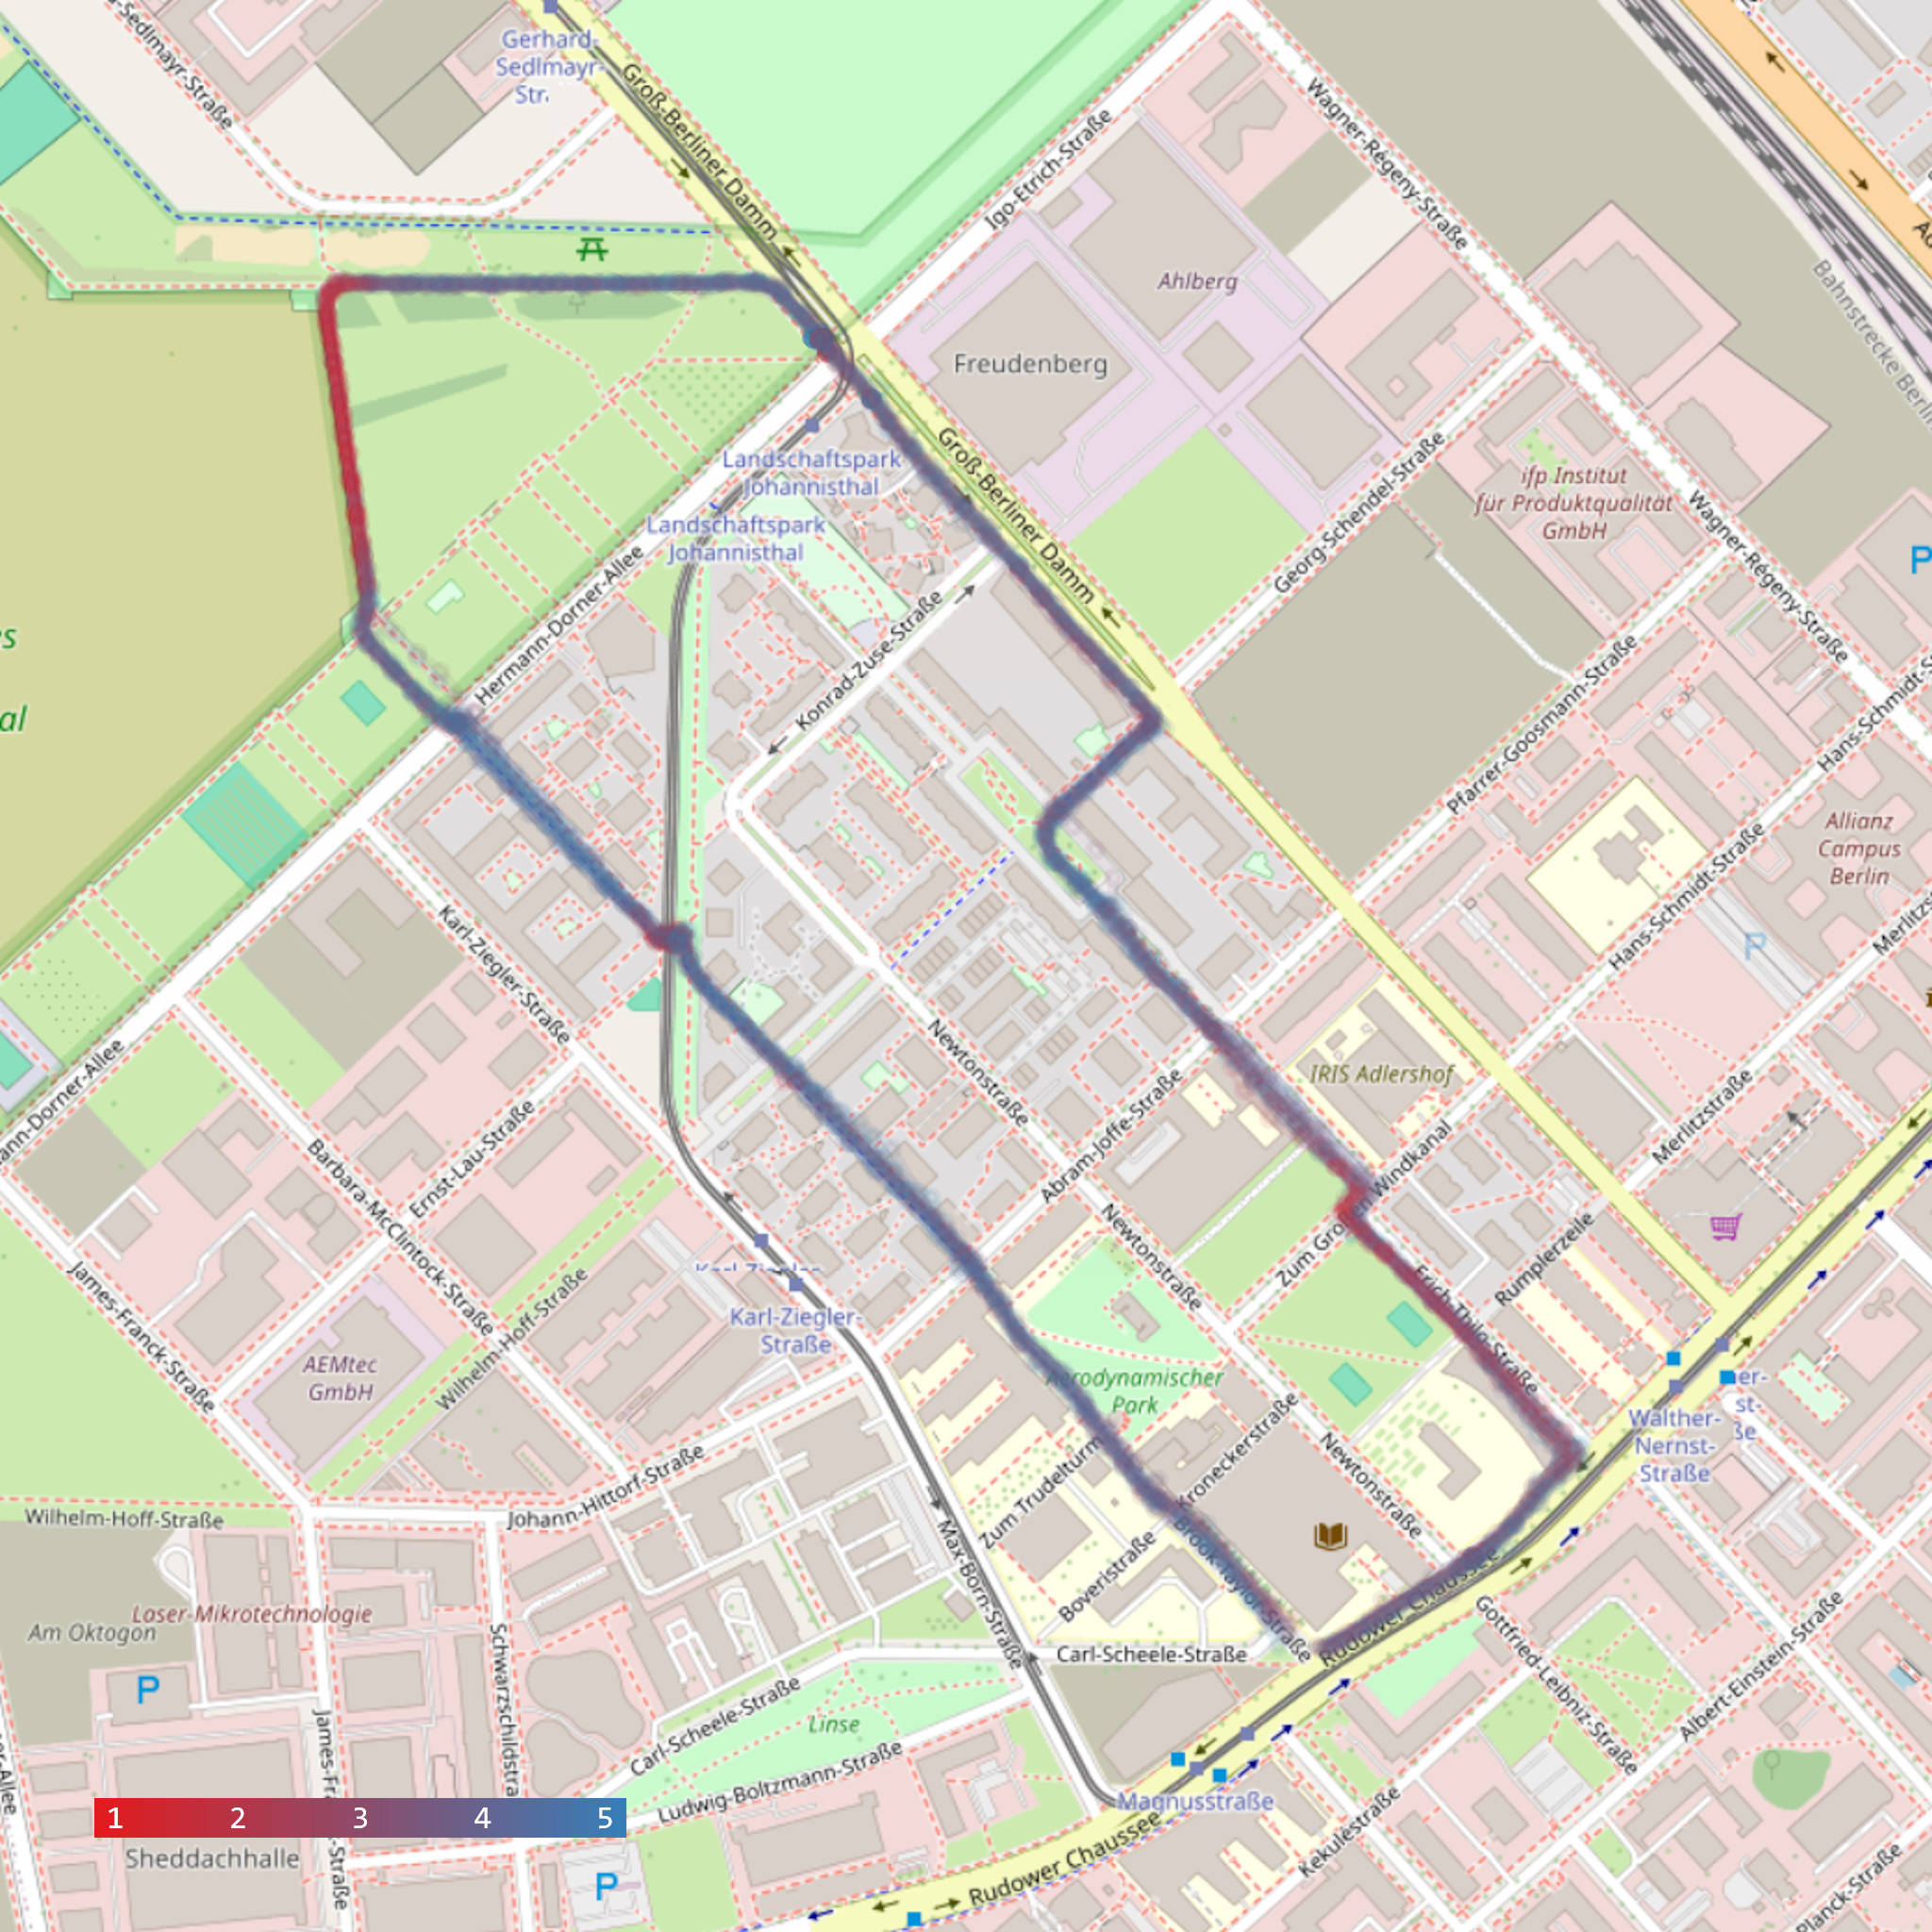
\includegraphics[width=.9\linewidth]{images/ratings_north_route.jpg}
        \caption{North route}
        \label{fig:ratings_north_route}
    \end{subfigure}%
    \begin{subfigure}{.3333\textwidth}
        \centering
        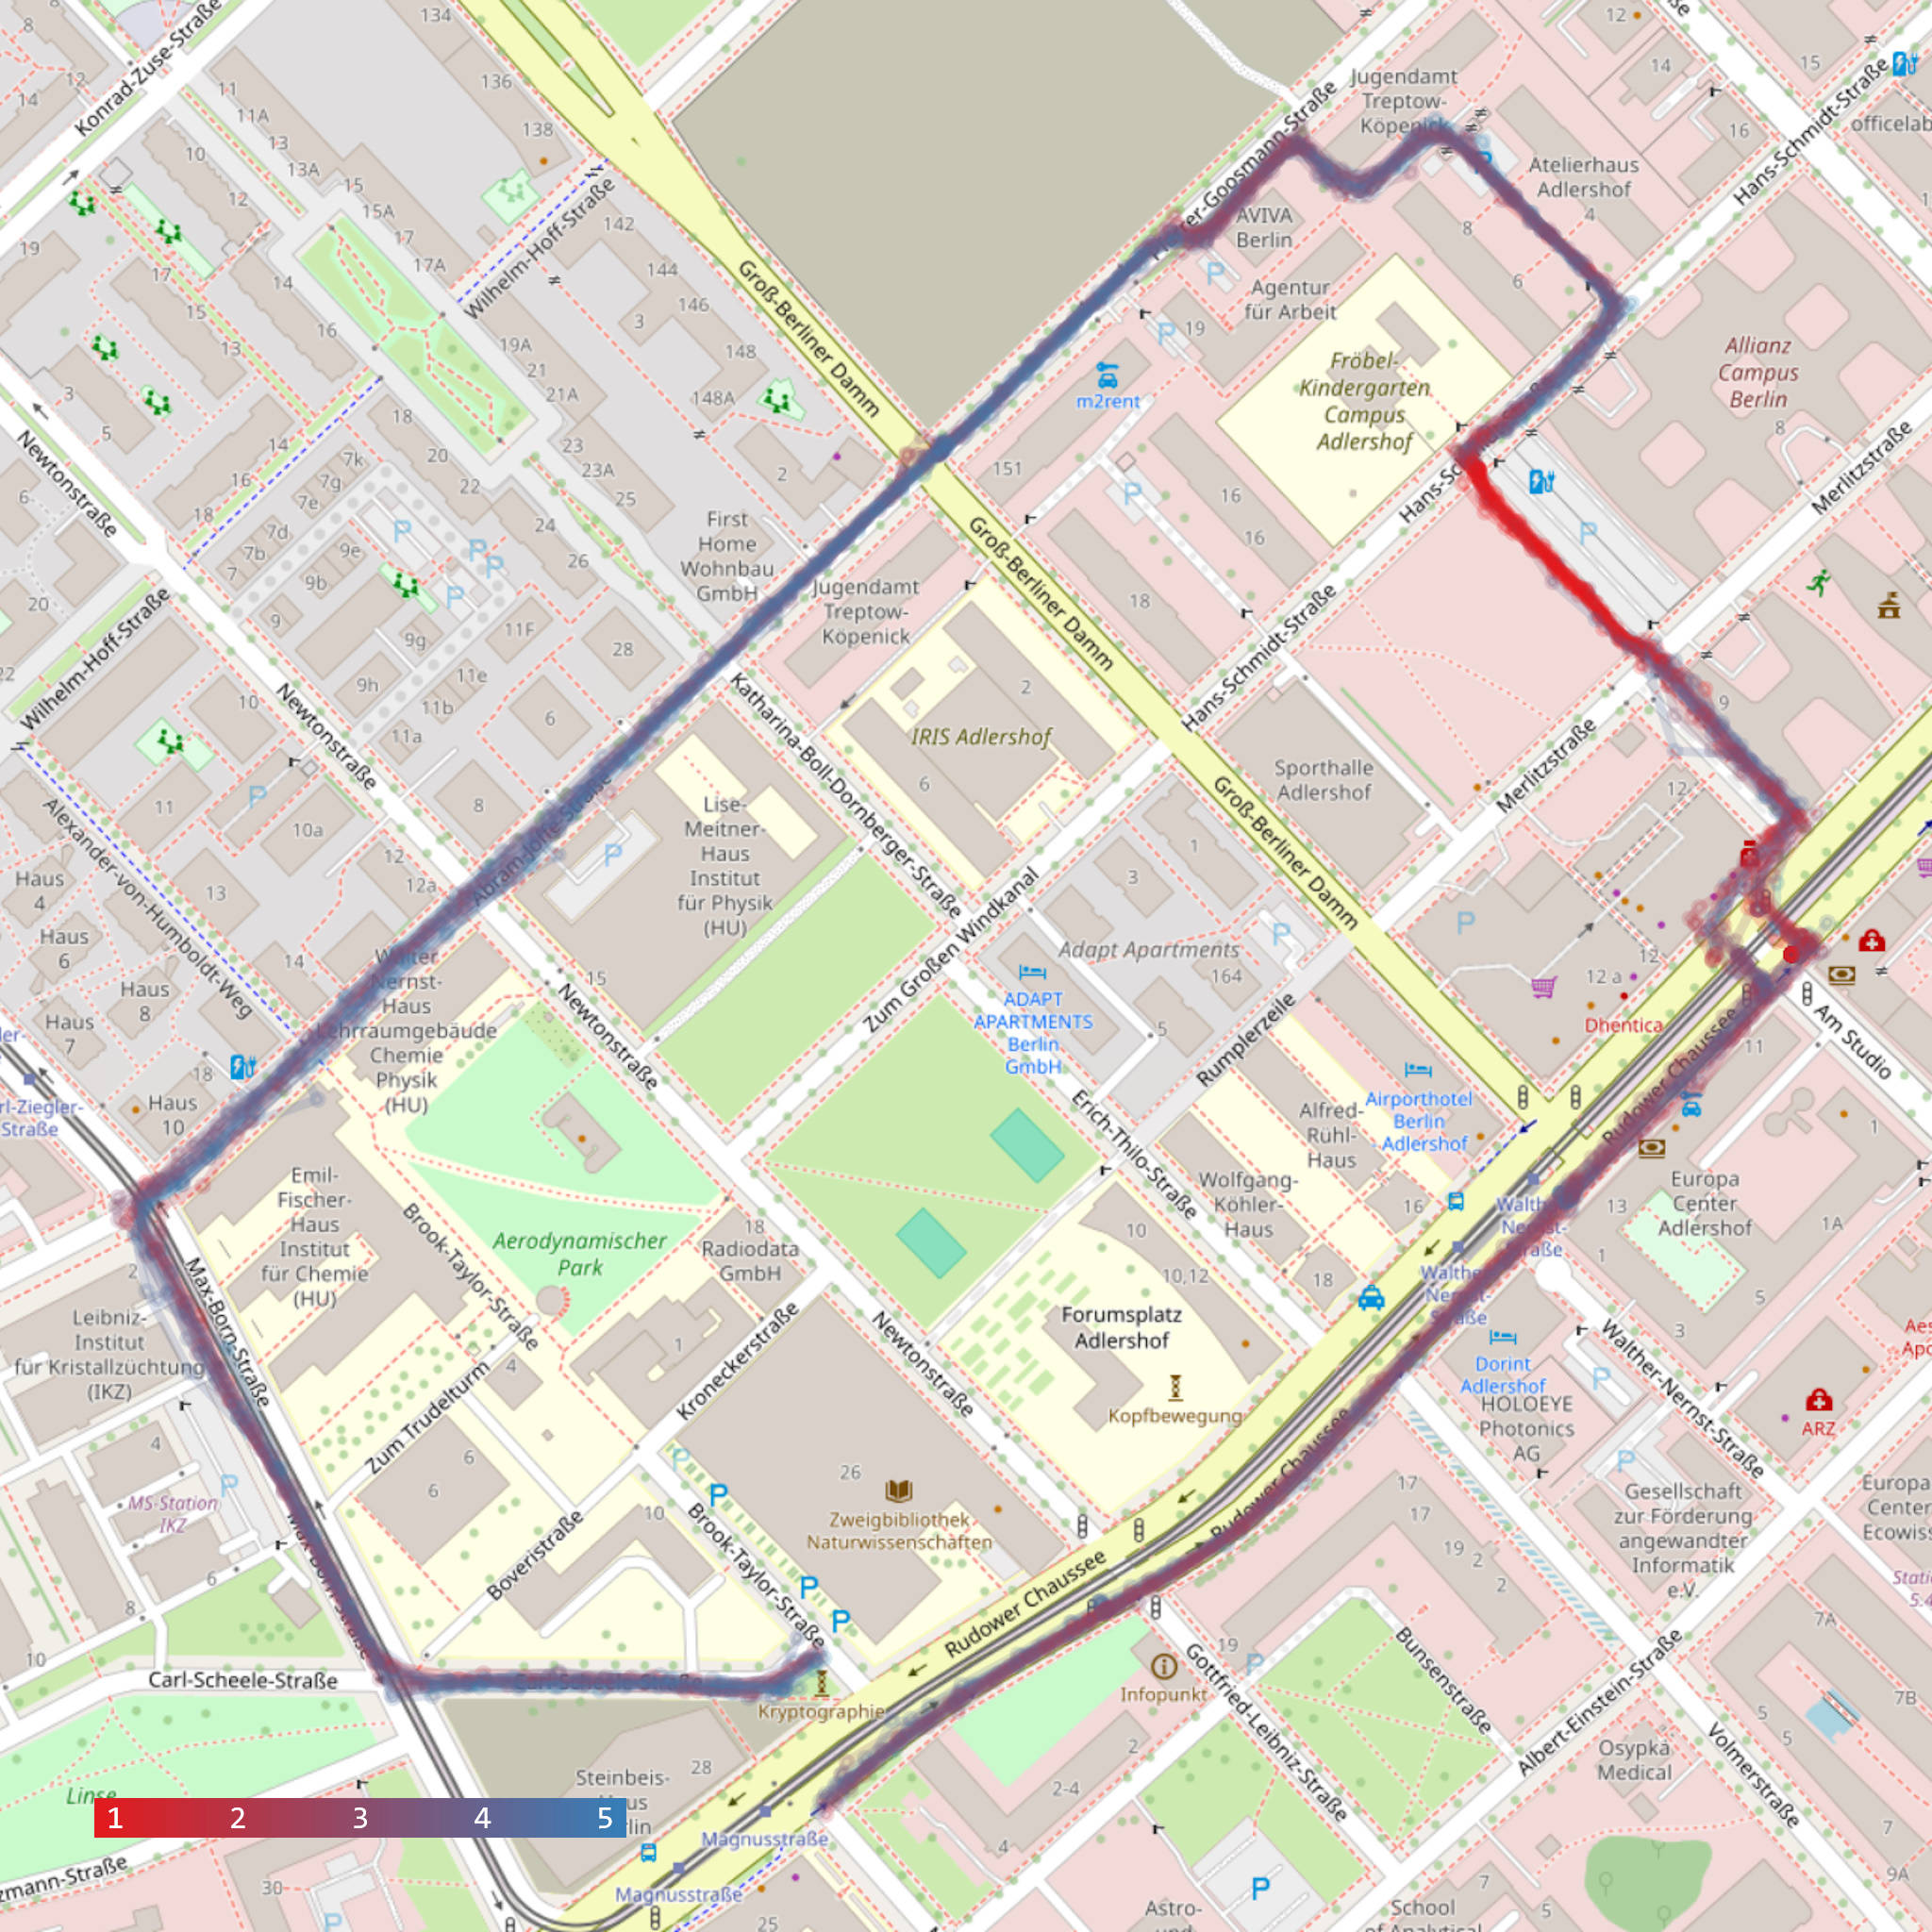
\includegraphics[width=.9\linewidth]{images/ratings_east_route.jpg}
        \caption{East route}
        \label{fig:ratings_east_route}
    \end{subfigure}%
    \begin{subfigure}{.3333\textwidth}
        \centering
        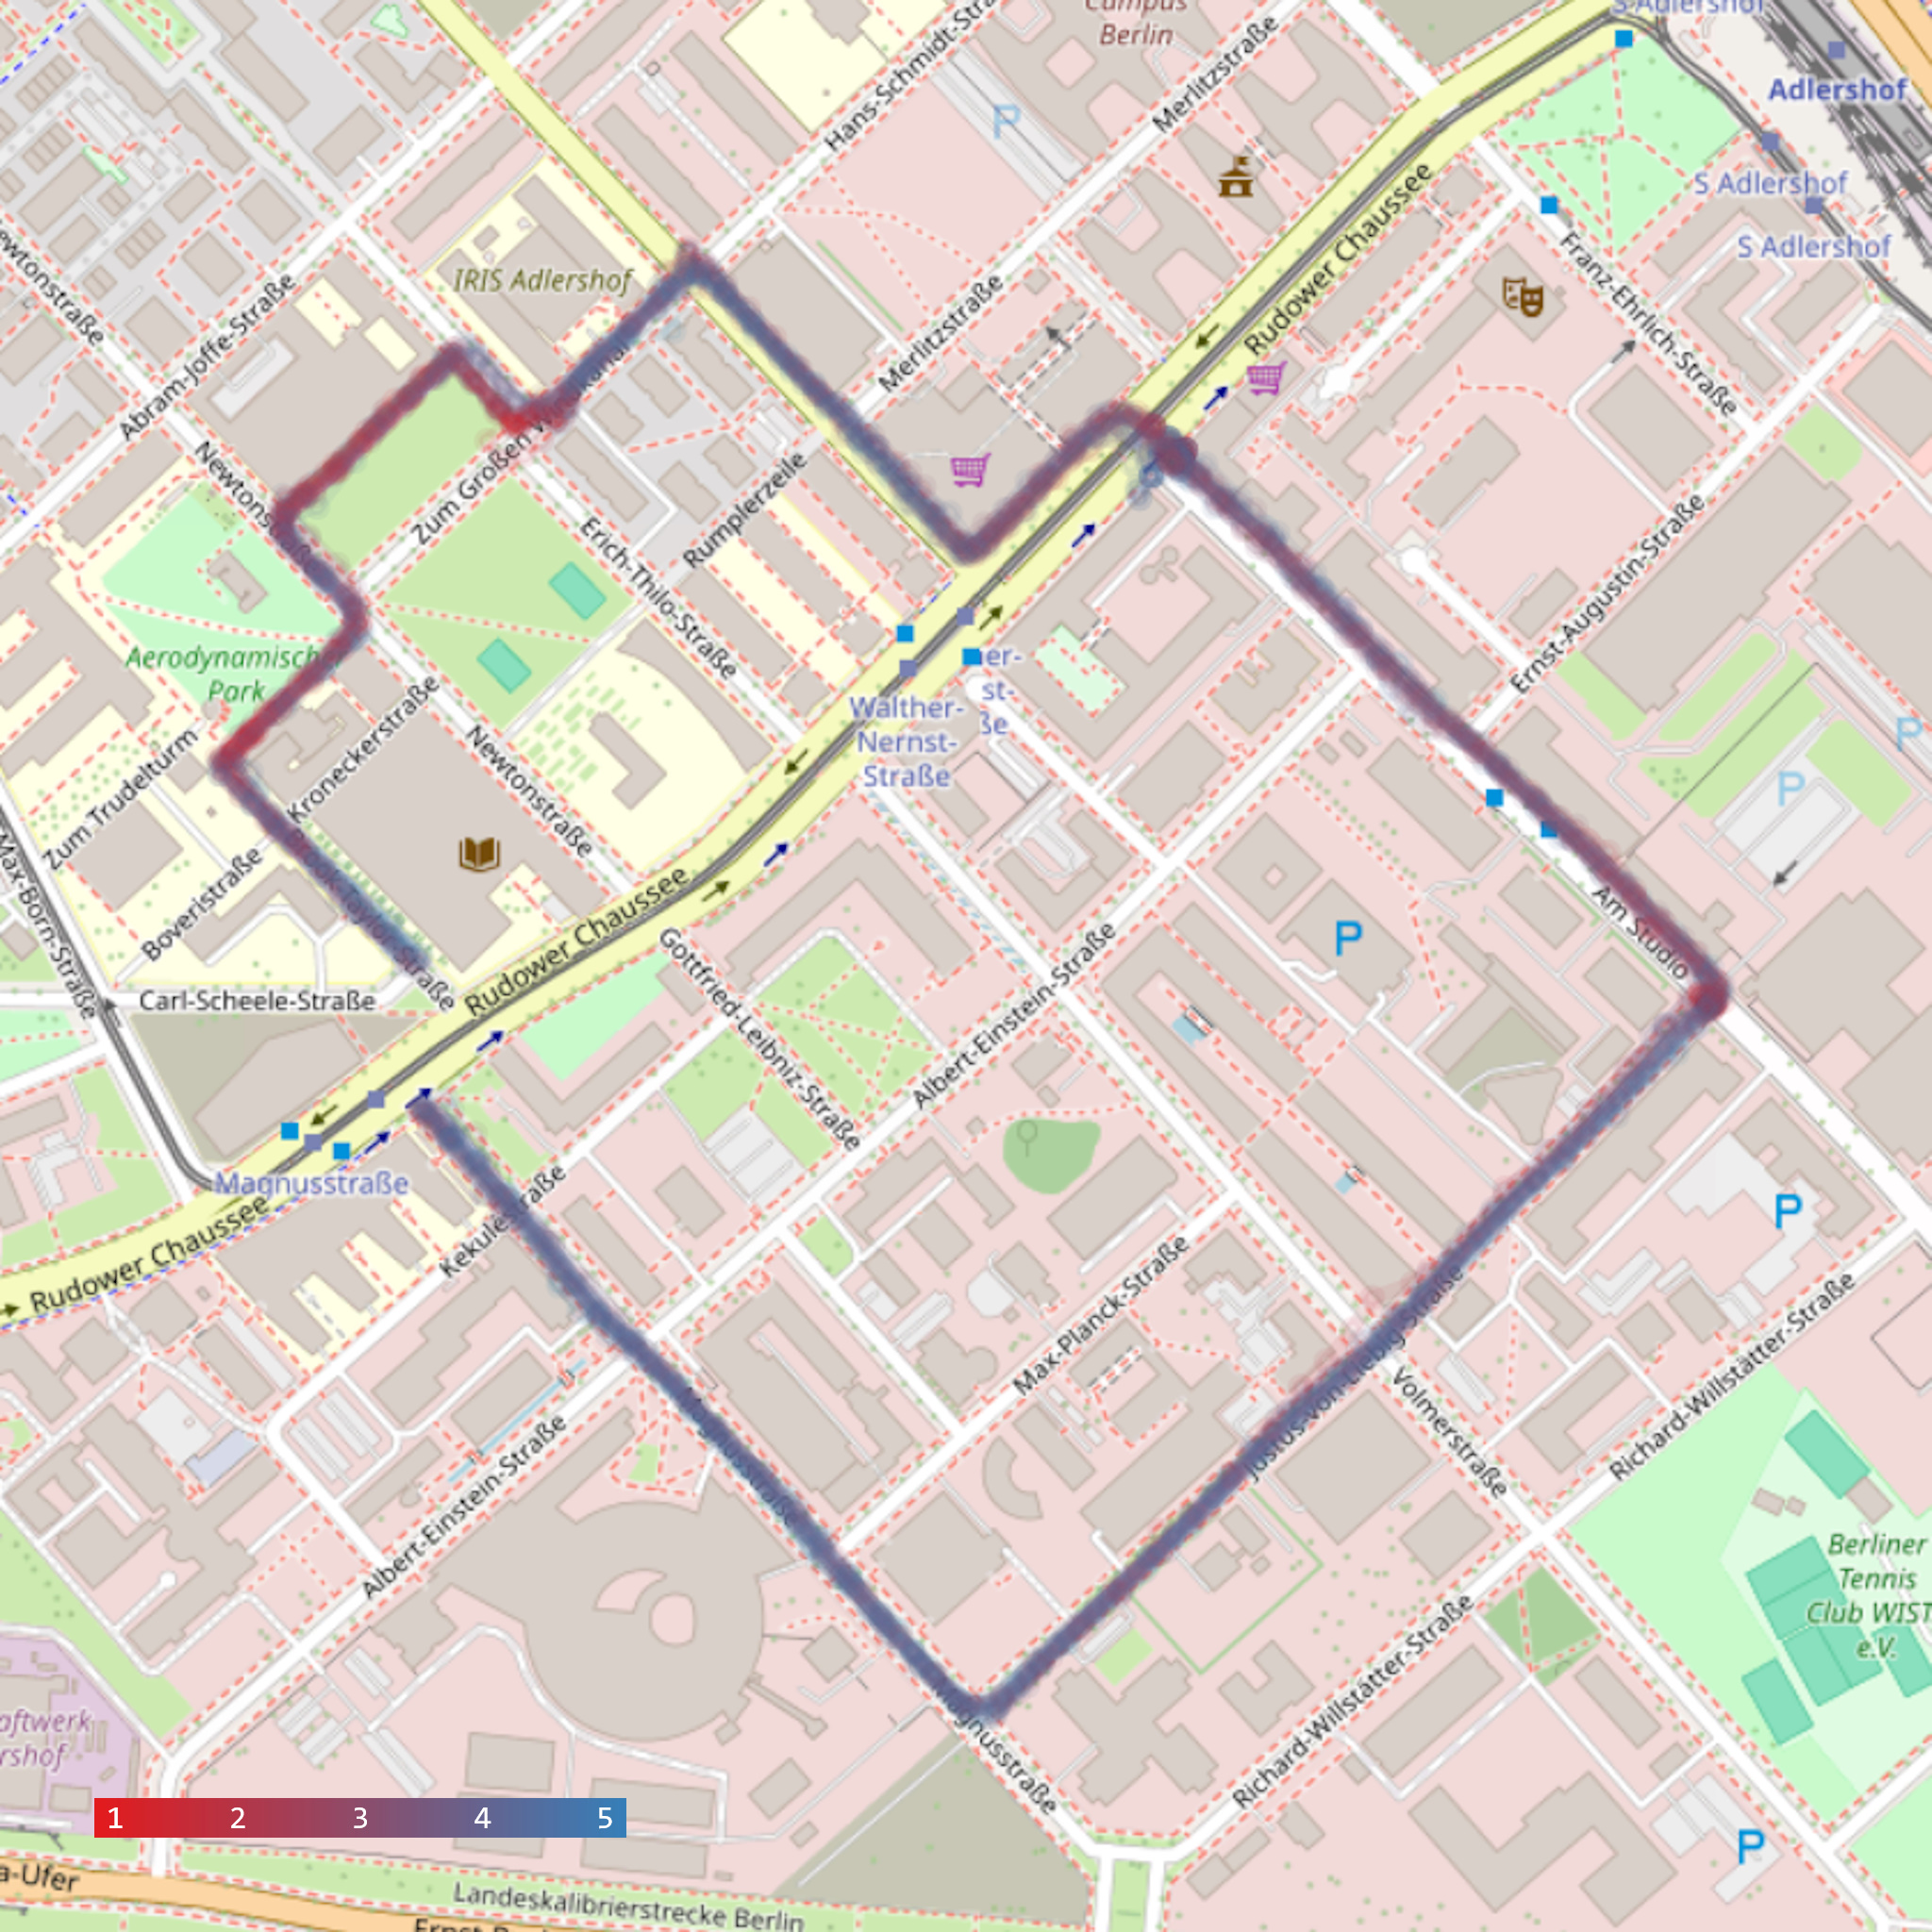
\includegraphics[width=.9\linewidth]{images/ratings_south_route.jpg}
        \caption{South route}
        \label{fig:ratings_south_route}
    \end{subfigure}\
    \caption{Combined ratings from all methods}
    \label{fig:route_ratings}
\end{figure}

\subsubsection{Preprocessing}\label{subsec:preprocessing}

Preprocessing of the recorded data was largely performed by hand, with the help of some simple python scripts.
The start and end position of all data recordings were adjusted manually, to remove unneeded data.
For the \audiorecording method, we had to manually listen to each audio file and extract the ratings performed by participants to match them to the recorded timestamps and GPS locations.
A similar process was used for the \mapping method to match the sections drawn on the paper maps to the recorded data.
Our \likertshift method required no further preprocessing.

\subsubsection{Evaluation}

As mentioned in \autoref{subsec:recording_methods}, comparing subjective data is inherently hard.
To perform our analysis, we categorized our original reference routes by road type and resampled them to $\sim\SI{1}{m}$ segments.
Then, we projected all recorded data from each method to them.
This left us with a combination of rating and road-type for each $\SI{1}{m}$ segment of each recording.
We then gathered all ratings by road-type for each method and computed their mean value, variance, and standard deviation, to see if we could see any drastic differences (see \autoref{table:likertshift_eval}).

\begin{table}[!htb]
    \footnotesize
    \centering
    \begin{tabular}{l|ccccccc}
        \multirow{2}{*}{\likertshift} & \multicolumn{7}{c}{Road Type}\\
        \cline{2-8}
        &&&&&&&\\[-1em]
        & Road & Bike Path & Mixed Path & Pedestrian Way & Wood Path & Field & Lawn\\[0.15em]
        \hline
        &&&&&&&\\[-0.8em]
        MEAN     & 3.7661 & 3.4624 & 3.7708 & 3.0176 & 1.8114 & 1.9804 & 2.8664\\[0.3em]
        VARIANCE & 0.9327 & 0.9140 & 0.8548 & 0.8873 & 0.9661 & 1.2512 & 1.3830\\[0.3em]
        STDDEV   & 0.9658 & 0.9560 & 0.9246 & 0.9420 & 0.9829 & 1.1186 & 1.1760\\
    \end{tabular}

    \vspace{1em}
    \begin{tabular}{l|ccccccc}
        \textsf{Audio} & \multicolumn{7}{c}{Road Type}\\
        \cline{2-8}
        &&&&&&&\\[-1em]
        \textsf{Recording} & Road & Bike Path & Mixed Path & Pedestrian Way & Wood Path & Field & Lawn\\[0.15em]
        \hline
        &&&&&&&\\[-0.8em]
        MEAN     & 3.6622 & 3.4978 & 3.7915 & 2.9559 & 2.5513 & 1.6895 & 2.4405\\[0.3em]
        VARIANCE & 0.8519 & 0.7970 & 0.8172 & 1.4158 & 0.5622 & 1.2402 & 0.9290\\[0.3em]
        STDDEV   & 0.9230 & 0.8927 & 0.9040 & 1.1899 & 0.7498 & 1.1137 & 0.9638\\
    \end{tabular}

    \vspace{1em}
    \begin{tabular}{l|ccccccc}
        \multirow{2}{*}{\mapping} & \multicolumn{7}{c}{Road Type}\\
        \cline{2-8}
        &&&&&&&\\[-1em]
        & Road & Bike Path & Mixed Path & Pedestrian Way & Wood Path & Field & Lawn\\[0.15em]
        \hline
        &&&&&&&\\[-0.8em]
        MEAN     & 3.7476 & 3.4952 & 3.7230 & 3.3553 & 2.3586 & 1.0000 & 3.0291\\[0.3em]
        VARIANCE & 0.9192 & 1.0542 & 1.0379 & 1.2773 & 1.5566 & 0.0000 & 1.0891\\[0.3em]
        STDDEV   & 0.9587 & 1.0267 & 1.0188 & 1.1302 & 1.2476 & 0.0000 & 1.0436\\
    \end{tabular}
    \caption{Evaluation of the recorded quantitative data}
    \label{table:likertshift_eval}
\end{table}

\subsection{Questionnaires and Interviews}

We evaluated each component of the \citetextnoref{nasa_tlx}{TLX} and \citetextnoref{ueq+}{UEQ+} surveys separately, without computing an overall index, because we are most interested in what components cause increased task load or affect the user experience.

The \textit{Physical Demand}, \textit{Temporal Demand}, and \textit{Performance} metrics of the \citetextnoref{nasa_tlx}{TLX} showed little statistical evidence for differences between methods.
The most notable difference is the increased \textit{Mental Demand} objected by the \mapping method, as well as higher \textit{Frustration} and perceived \textit{Effort} in comparison to the live-recording methods.
There is insufficient statistical evidence for differences in task load between our \likertshift method and the \audiorecording method.

\begin{figure}[!htb]
    \centering
    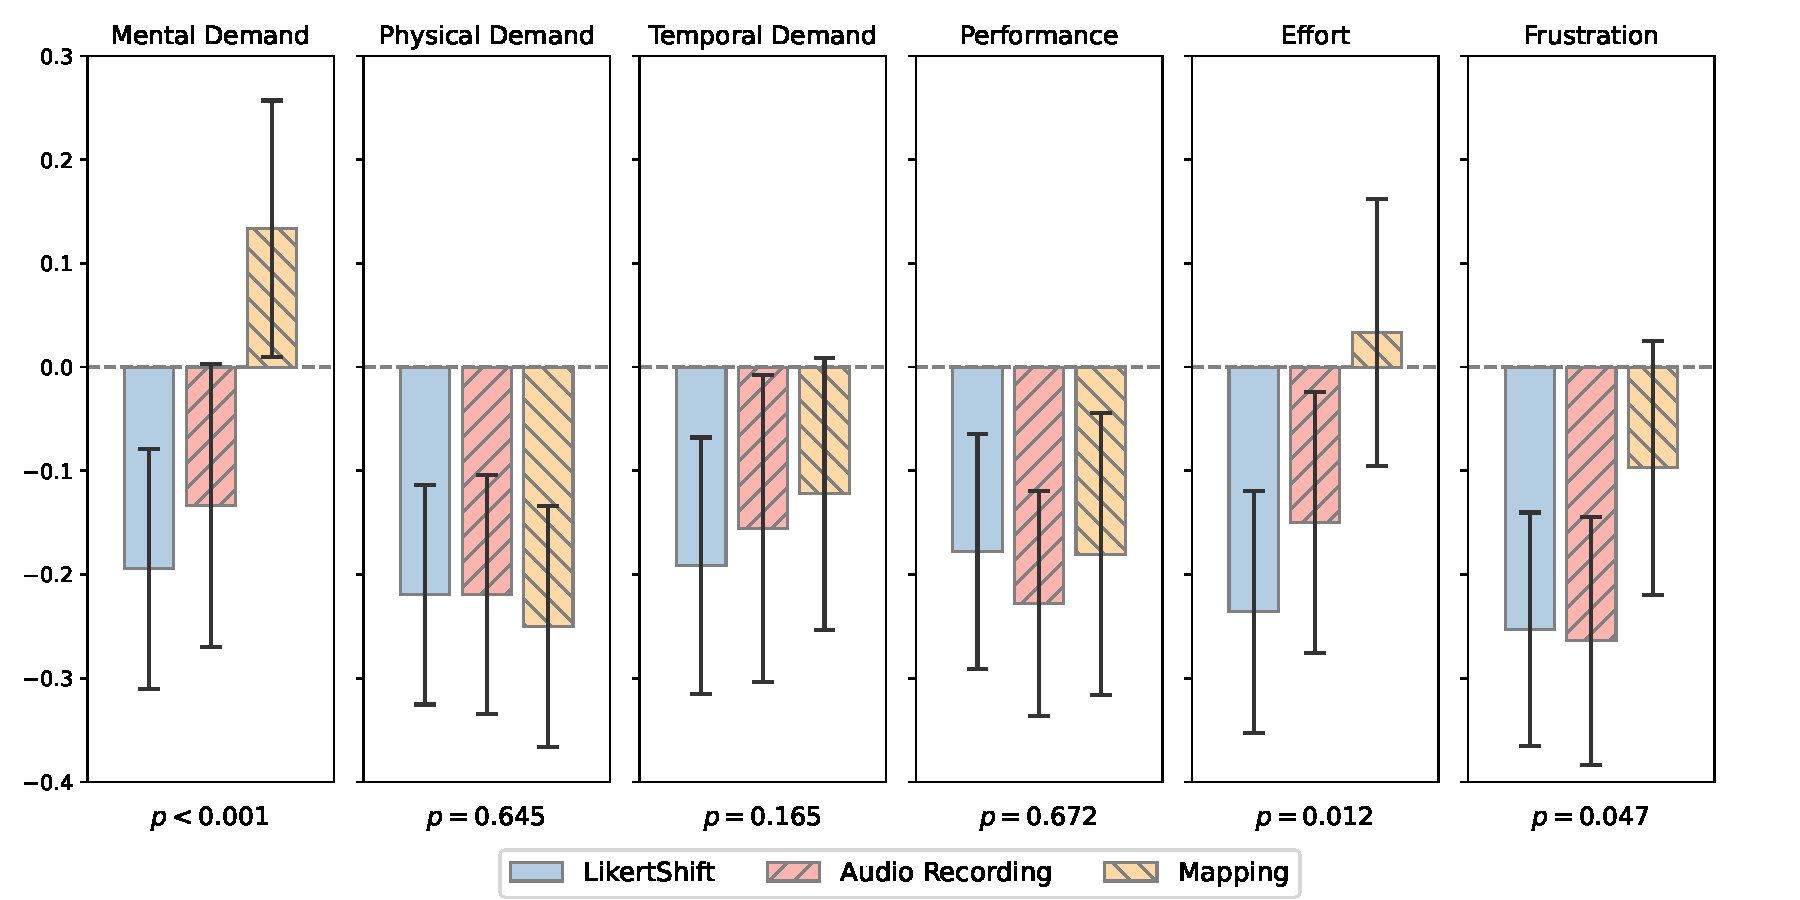
\includegraphics[height=0.5\linewidth]{../evaluation/eval_tlx.pdf}
    \caption{TLX results (the errorbars denote the confidence interval based on a student's distribution; $p$ values are computed using a Friedman test; values are normalized from -1 to 1)}
    \label{fig:eval_tlx}
\end{figure}

\bigbreak\noindent
The evaluation of the \citetextnoref{ueq+}{UEQ+} metrics turned out to be more interesting.
We observed incredibly evidence for the \textit{Attractiveness} and \textit{Intuitiveness} of our \likertshift method, compared to the other ones.
While participants perceived the \likertshift and \audiorecording methods to be similarly \textit{Efficient}, in comparison, the \mapping method was perceived as highly inefficient.
We can also observe low \textit{Social Acceptance} ratings of the \audiorecording method.

These findings were confirmed by our performed interviews.
Multiple participants denoted that the additional time requirements of the \mapping method make using it very unattractive to them.
Similarly, the majority of participants stated they did not like to talk during cycling and found it “awkward” to perform the \audiorecording method.
When asked what method participants would choose to conduct a longer ($\sim\SI{2}{weeks}$) field-study which would require them to record their travel satisfaction on all of their commutes and other trips, 17 out of 18 participants chose our \likertshift method.

\begin{figure}[!htb]
    \centering
    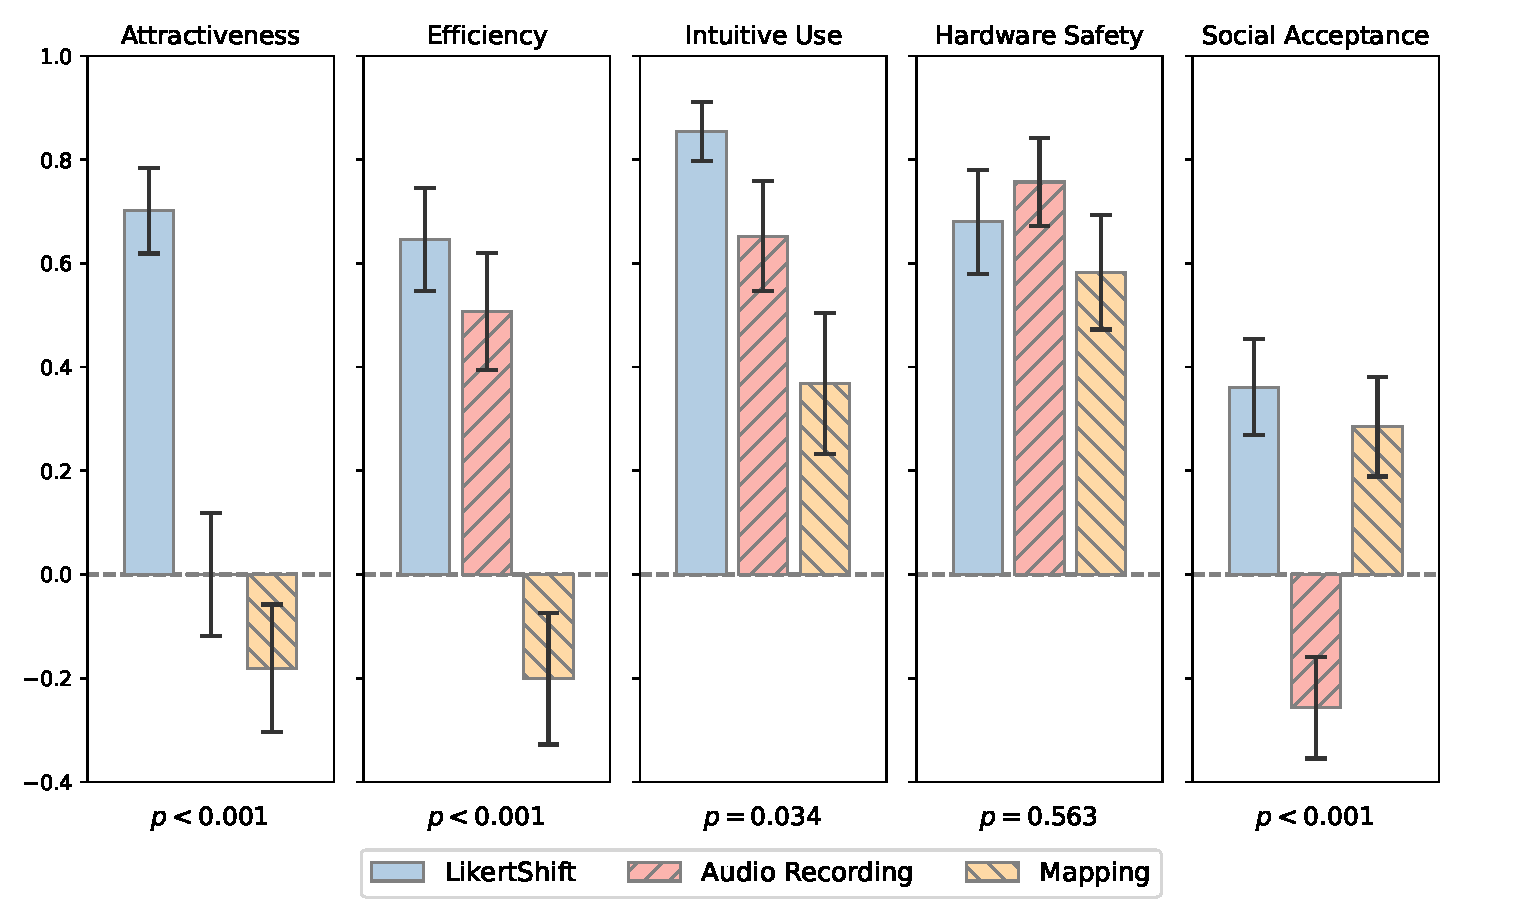
\includegraphics[height=0.5\linewidth]{../evaluation/eval_ueq.pdf}
    \caption{UEQ+ results (the errorbars denote the confidence interval based on a student's distribution; $p$ values are computed using a Friedman test; values are normalized from -1 to 1)}
    \label{fig:eval_ueq}
\end{figure}
